\documentclass[12pt]{article} % Article with 12pt font
% Set font to Times
\usepackage[T1]{fontenc}
\usepackage[utf8]{inputenc}
\usepackage{mathptmx}

% Double spacing
\usepackage{setspace}
\doublespacing

% Paper size and margins
\usepackage[letterpaper, margin=1in]{geometry}

% Float placement control
\usepackage{float}

% Special symbols
\usepackage{gensymb}

% Extra math notation
\usepackage{amsmath}

% Include graphics
\usepackage{graphicx}

% sub-figures with sub-labels
\usepackage{subcaption}

% Number tables with Roman numerals
\renewcommand{\thetable}{\Roman{table}}

% Section header formatting
\usepackage{sectsty}
\sectionfont{\centering\normalsize}
\subsectionfont{\normalsize}
\subsubsectionfont{\underline\normalfont\normalsize}

\begin{document}
\fontfamily{ptm}\selectfont % Turn Times font on

%------------------------------------------------------------------------------------------------%
\begin{titlepage}
    \begin{center}
        \large

        \vspace*{1.5in}
        AE 3610, Lab \#42

        \vspace{1.5in}
        \textbf{An Experiment Conducted with Poorly Functioning Apparatus}

        \vspace{0.5in}
        By: \textbf{G. P. Burdell}

        \vspace{2in}
        Group I1

        \vspace{0.5in}
        Fall Semester 2019
    \end{center}
\end{titlepage}
%------------------------------------------------------------------------------------------------%
%------------------------------------------------------------------------------------------------%
\section*{Introduction}
Sample text.
%------------------------------------------------------------------------------------------------%
%------------------------------------------------------------------------------------------------%
\section*{Data Results}
%------------------------------------------------------------------------------------------------%
\subsection*{Raw Data}
%------------------------------------------------------------------------------------------------%
Sample text.
%------------------------------------------------------------------------------------------------%
\subsection*{Reduced Data}
%------------------------------------------------------------------------------------------------%
Sample text.
%------------------------------------------------------------------------------------------------%
%------------------------------------------------------------------------------------------------%
\section*{Discussion}
%------------------------------------------------------------------------------------------------%
\subsection*{Answers to Supplement Questions}
%------------------------------------------------------------------------------------------------%
\subsubsection*{Question 1}
Sample text.
\subsubsection*{Question 2}
Sample text.
\begin{equation}
    \label{eq:f}
    f(u)
\end{equation}
%------------------------------------------------------------------------------------------------%
\subsection*{Additional Discussion}
%------------------------------------------------------------------------------------------------%
See Equation (\ref{eq:f}), Figure \ref{fig:bar}, and Table \ref{tab:foo}.
Sample $c + \vec{K}$ text.
%------------------------------------------------------------------------------------------------%
%------------------------------------------------------------------------------------------------%
\section*{Tables and Figures}
%------------------------------------------------------------------------------------------------%
\begin{table}[H]
    \centering
    \caption{Some data that's probably wrong.}
    \label{tab:foo}
    \begin{tabular}{ c  c }
        \hline
        \textbf{First Column} & \textbf{Second Column}\\
        \hline
        0.42 & 4.2 \\
        \hline
    \end{tabular}
\end{table}

\begin{figure}[H]
    \centering
    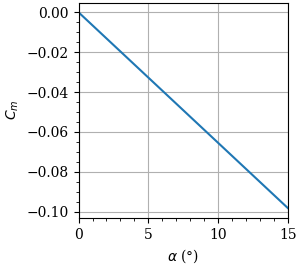
\includegraphics[width=\linewidth]{plot.png}
    \caption{A graph to prove how wrong the data is.}
    \label{fig:bar}
\end{figure}
%------------------------------------------------------------------------------------------------%

\end{document}
